\documentclass{article}
\usepackage[utf8]{inputenc}
\usepackage[margin=1in]{geometry}
\usepackage{graphicx}

\title{Math Clinic Status Update 3}
\author{Team 1: Komi Agbo, Dalton Burke, Nick Mako, James Vance}
\date{November 11th, 2019}

\begin{document}

\maketitle

\section{Since our last update...}
We have integrated the data that the professor published, and compared the 
outcomes for inter-zone delivery-pickup pairs allowed, and not allowed. In
this instance, the differences of the times for the total routes (without
transitions) is about 70 minutes (out of around 1600 minutes) over the whole
day, across 8 drivers. With the added complexity of extra transitions, it seems
like we would probably do better to keep delivery-pickup pairs restricted to 
the same zone.

\begin{center}
	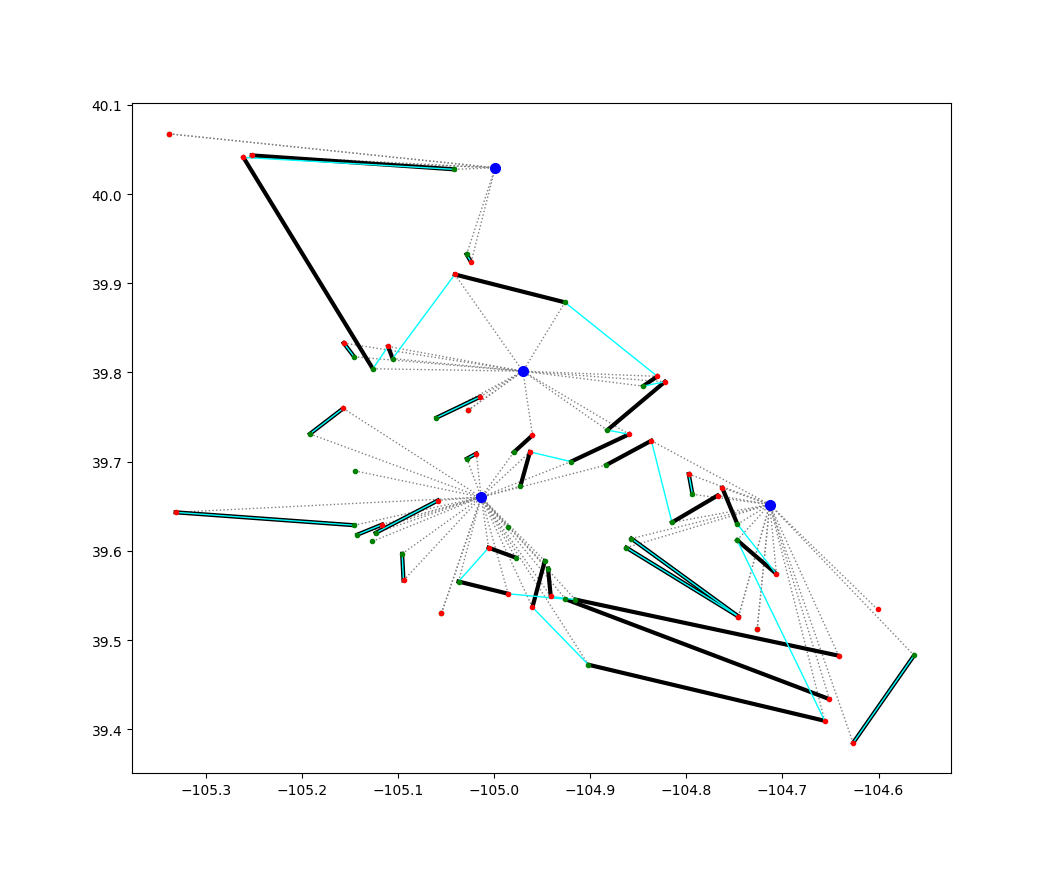
\includegraphics[scale=.55]{img/real_data_matching.png}\\
	Matching visualization with actual customer data. Cyan edges are when
	delivery-pickup pairs are zone restricted, and black edges are when
	they may cross zones.
\end{center}

Interestingly, preliminary results from the route assignment algorithm (which
we have also been working on) are showing that it may still be better to use
the interzone matching, even with the overhead of less efficient transitions.
However, at this stage we aren't completely sure that the results of the route
assignment are valid.

\section{What's on our plate now...}
\begin{itemize}
  \item Work more on making good transitions
  \item Visualize route assignments
\end{itemize}
\section{What's next...}
\begin{itemize}
  \item Satisfy other constraints for driver routes
  \item Satisfy inventory constraints for landfills
\end{itemize}

\end{document}

